\documentclass[../../main.tex]{subfiles}

\begin{document}

\subsection{Motivation}
There are several well-known tensor decomposition methods, but there is no clear understanding how they compare in terms of quality. 

In this work we aim to compare different high-order tensor decomposition techniques, provided in HottBox\footnote{\url{https://hottbox.github.io/stable/index.html}} tooling. More specifically, we benchmark CPD, Tucker Decomposition and Tensor-Train against three quality criterions: precision, stability and computational complexity.

As an input data we use Tensor Flow logo (three dimensional tensor). For this tensor we find low-rank approximations and then calculate quality criterions listed above.


\subsection{Problem statement}

Formally, let's state $X$ is an 3rd order tensor (input image). We define approximations in the following way:


\begin{equation} \label{eq:kotua_1}
\underline{\mathbf{X}}=\sum_{r=1}^{R} \underline{\mathbf{X}}_{r}=\sum_{r=1}^{R} \lambda_{r} \cdot \mathbf{a}_{r} \circ \mathbf{b}_{r} \circ \mathbf{c}_{r} \end{equation}


\begin{equation} \label{eq:kotua_2}
\underline{\mathbf{X}}=\underline{\mathbf{G}} \times_{1} \mathbf{A} \times_{2} \mathbf{B} \times_{3} \mathbf{C}\end{equation}


\begin{equation} \label{eq:kotua_3}
\underline{\mathbf{X}}=\mathbf{A} \times{ }_{2}^{1} \underline{\mathbf{G}}^{(1)} \times_{3}^{1} \underline{\mathbf{G}}^{(2)} \times_{3}^{1} \cdots \times_{3}^{1} \underline{\mathbf{G}}^{(N-1)} \times_{3}^{1} \mathbf{B}\end{equation}

Where \ref{eq:kotua_1} - \ref{eq:kotua_3} correspond to CPD, HOSVD and Tensor-Train decompositions. Corresponding output tensors we define as $X_{cpd}, X_{ho}, X_{tt}$.

Precision is defined the following way:

\begin{equation}
    Precision = \frac{|X - X_i|}{|X|},  \forall i \in \set{\{cpd, ho, tt\}}
\end{equation}

Complexity is calculated as time taken to complete decomposition. Stability is estimated as increase in error when some Gaussian noise is added to the input tensor. In this work Gaussian noise is a tensor of same shape as X, where each element is sampled from the normal distribution with parameters $\mu$ and $\sigma$.

\subsection{Experiment description}

Tensor Flow logo is taken as an input image. The input converted to the 3rd order tensor with shape (232, 217, 4). 

Then, three experiments are conducted for each type of tensor decomposition (CPD, HOSVD and Tensor Train):

\begin{enumerate}
    \item Calculate relative error of decomposition for different ranks of core tensor
    \item Measure time taken to compute the decomposition for each of the rank
    \item Calculate relative error of decomposition when Gaussian noise with different sigma is added to the input image. Repeat it for each rank and then plot 3D graph, illustrating the stability.
\end{enumerate}

\subsection{Plots and analysis}

First of all, we compare how relative error decreases with regards to the rank for different tensor decompositions. As it can be seen from the chart \ref{fig:kotua:2}, TT and HOSVD showcase almost identical results while CPD is quite noisy and its errors decrease slower.

\begin{figure}[h!]
\centering
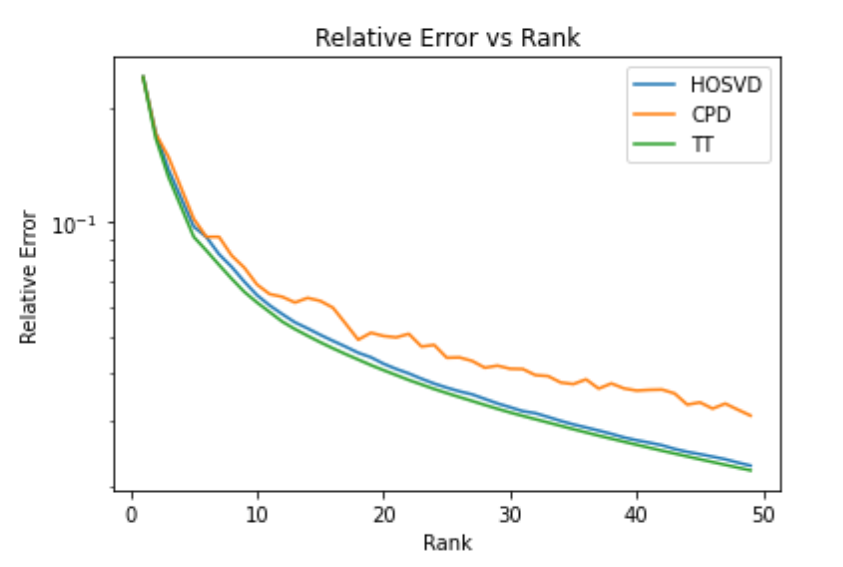
\includegraphics[width=0.6\textwidth]{figures/errors}
\caption{Comparison of relative error of decomposition w.r.t rank for HOSVD, CPD and TT.}
\label{fig:kotua:2}
\end{figure}

In terms of the computational complexity, HOSVD is a clear leader. CPD, on the other hand, is again an outsider. On the chart \ref{fig:kotua:3} the time axis is plotted in the logarithmic scale, so it can be seen, that CPD is slower than HOSVD by a factor of 100.

\begin{figure}[h!]
\centering
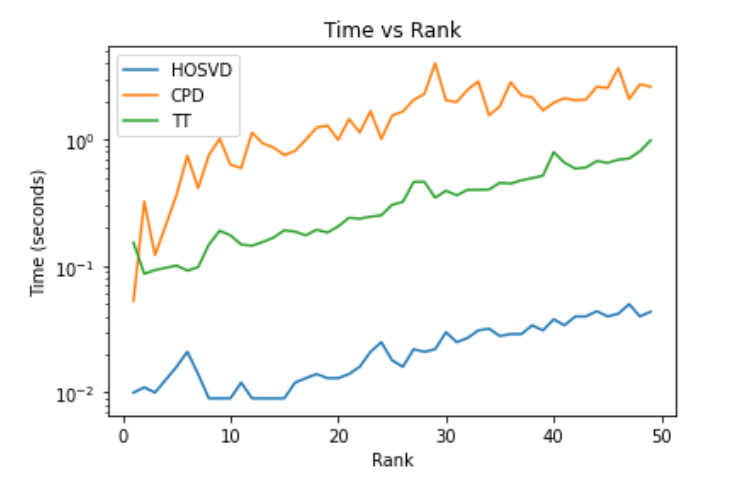
\includegraphics[width=0.6\textwidth]{figures/times}
\caption{Comparison of complexity of decomposition w.r.t rank for HOSVD, CPD and TT.}
\label{fig:kotua:3}
\end{figure}

\subsubsection{Noisy Data}

Charts \ref{fig:kotua:4} - \ref{fig:kotua:6} show, how noise influences stability of algorithms. In general, algorithms behave identically: the error decreases with regards to rank when noise is insignificant. But when noise becomes large errors start to increase with regards to rank.

\begin{figure}[h!]
\centering
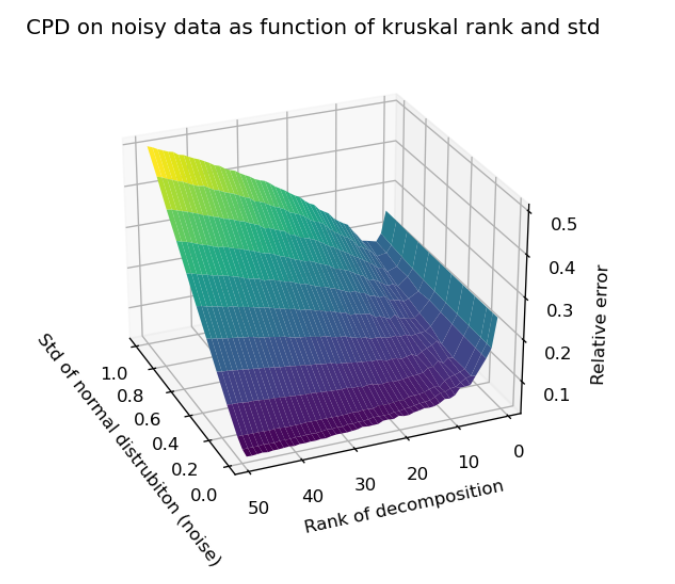
\includegraphics[width=0.6\textwidth]{figures/cpd}
\caption{Relative error of CPD decomposition w.r.t to rank and standard deviation of Gaussian noise.}
\label{fig:kotua:4}
\end{figure}

Interestingly enough, regardless of noise amplitude, at low ranks errors decrease before reaching some threshold. After that point the growth trend takes its lead.

\begin{figure}[h!]
\centering
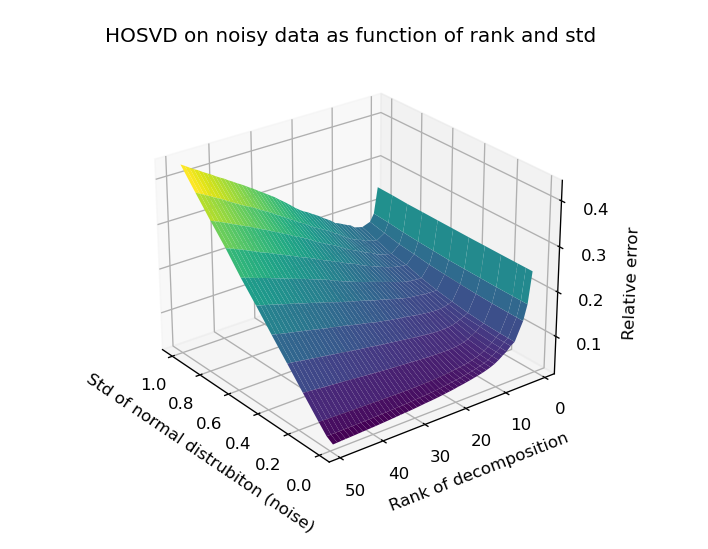
\includegraphics[width=0.6\textwidth]{figures/hosvd}
\caption{Relative error of HOSVD decomposition w.r.t to rank and standard deviation of Gaussian noise.}
\label{fig:kotua:5}
\end{figure}

\begin{figure}[h!]
\centering
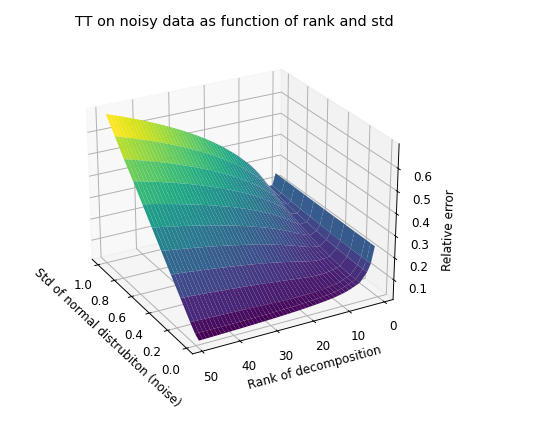
\includegraphics[width=0.6\textwidth]{figures/tt}
\caption{Relative error of TT decomposition w.r.t to rank and standard deviation of Gaussian noise.}
\label{fig:kotua:6}
\end{figure}

To summarize staiblity criterions, let's take a look on the chart \ref{fig:kotua:7}. It compares algorithms when small noise (std = 0.1) is added to the picture.As you can see from this chart, HOSVD is the most stable algorithm. CPD is also quite good at high ranks, but no so good at low ranks. Tensor Train is on par with HOSVD at low ranks, but it become less stable at high ranks.  

\begin{figure}[h!]
\centering
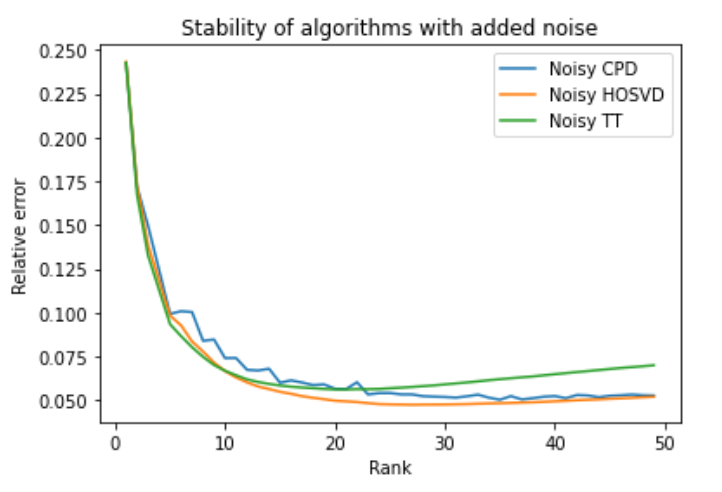
\includegraphics[width=0.6\textwidth]{figures/stability}
\caption{Relative error of TT decomposition w.r.t to rank and standard deviation of Gaussian noise.}
\label{fig:kotua:7}
\end{figure}

\subsection{Conclusion}
Judging by all three parameters (precision, stability and complexity) HOSVD is the best algorithm. It's very fast, stable and on par with Tensor Train in terms of precision. Tensor Train has a bit more accurate results, but it's definitely slower and not so stable. CPD is computationally expensive and its error decreases very slow with regards to rank. Though it is quite stable when it comes to high ranks.


\end{document}